\documentclass[../../main.tex]{subfiles}

\begin{document}

\subsubsection{Introduction}

In this iteration I will start working on the frontend, or the client application. The client
application will talk to the backend service I created in the previous iteration and will
provide the client with an intuitive user interface through which they can interact with the
backend service and by extension the database connected to it.

\noindent \\ The two applications, as I mentioned in the first iteration's introduction,
will communicate using GraphQL. The client application itself will make use of
React Native and Expo.

\noindent \\ React Native is an open-source user interface (UI) framework created by
Facebook which allows developers to easily write native applications using
the high-level JavaScript and TypeScript languages. This is opposed to the conventional method
of writing applications for these platforms where different apps would need to be programmed
in different languages for different systems (eg. Android, iOS). React Native allows code to
be written once in a high level language and subsequently executed on multiple
platforms without modification.

\noindent \\ Expo is an open-source SDK (\textbf{S}oftware \textbf{D}evelopment \textbf{K}it) designed to allow high-level code, such as code
written for React Native, to access low-level platform-specific features, such as a devices' camera.
It acts as an \textbf{abstraction layer} providing a generic interface to access such features.

\begin{comment}
\noindent \\ Therefore, the first task to do is to initialise an Expo project and install
our dependencies, notably the Apollo GraphQL client.\
\end{comment}

\subsubsection{Prototyping using the 'Expo Go' application}

Expo Go is a sandbox used to execute an Expo project without having to build it to a native application.
Expo Go can be installed from app-stores and connects to a server located
on another machine (Started using \lstinline{expo start}) which contains the source code.

\noindent \\ JavaScript is an interpreted language, but platform-specific components of both
the Expo SDK and React Native are written in a compiled language such as Java (Android) or Swift (iOS).
Expo Go works by providing a barebones application with the required native code already compiled,
so a server can simply host the remaining interpreted JavaScript code.

\noindent \\ For this iteration, I will use Expo Go for quick prototyping.
However, it is important to note that Expo Go does have it's limitations.
Namely, any dependencies requiring additional native code will not work in Expo Go.
I will need to be aware of this during development of this and future frontend iterations.

\subsubsection{Creating an Expo project}

There are two requirements to consider before creating an Expo project.
The first requirement is to install Node.js, the second to decide which Expo SDK version
to use. Node.js is a portable JavaScript runtime which is used to execute the tools necessary
to create an Expo project.

\noindent \\ Expo Go supports the last three Expo SDK releases.
I have chosen to use the latest SDK at the time of writing, SDK 50.
I chose this version as it introduces a new version of a core expo feature,
\lstinline{expo-router} version 3.

\noindent \\ To create an Expo project, assuming Node.js is installed, open a terminal and type:

% TODO: move to minted? 
% https://tex.stackexchange.com/questions/89276/insert-bash-code-with-coloration-into-my-latex-report
\begin{lstlisting}[language=bash]
    [james@linux cs-coursework]$ npx create-expo-app@latest fosscat-frontend --template tabs@50
\end{lstlisting}

\noindent Wait for the command to finish, and you will have the following output:

\begin{lstlisting}[language=bash]
Need to install the following packages:
create-expo-app@2.3.1
Ok to proceed? (y) y
> Downloaded and extracted project files.
> Your project is ready!

To run your project, navigate to the directory and run one of the following npm commands.

- cd fosscat-frontend
- npm run android
- npm run ios
- npm run web
\end{lstlisting}

\noindent \\ \lstinline{npx} is a Node.js command that allows us to execute the contents of a package,
installing the package if was not already available. We are executing the package \lstinline{create-expo-app}
with the argument \lstinline{fosscat-frontent} as the package name.
We are also making use of a \lstinline{expo-router} template, namely the "tabbed" template.
This means that create-expo-app will also generate boilerplate code for \lstinline{expo-router},
such as an initial home page (or route).

\noindent \\ This command sets up and creates an Expo project, including installing dependencies such as
React, React Native and TypeScript.

% Dummy env to escape wrapfig
\begin{dummyenv}

  \begin{wrapfigure}{r}{0.4\textwidth}
    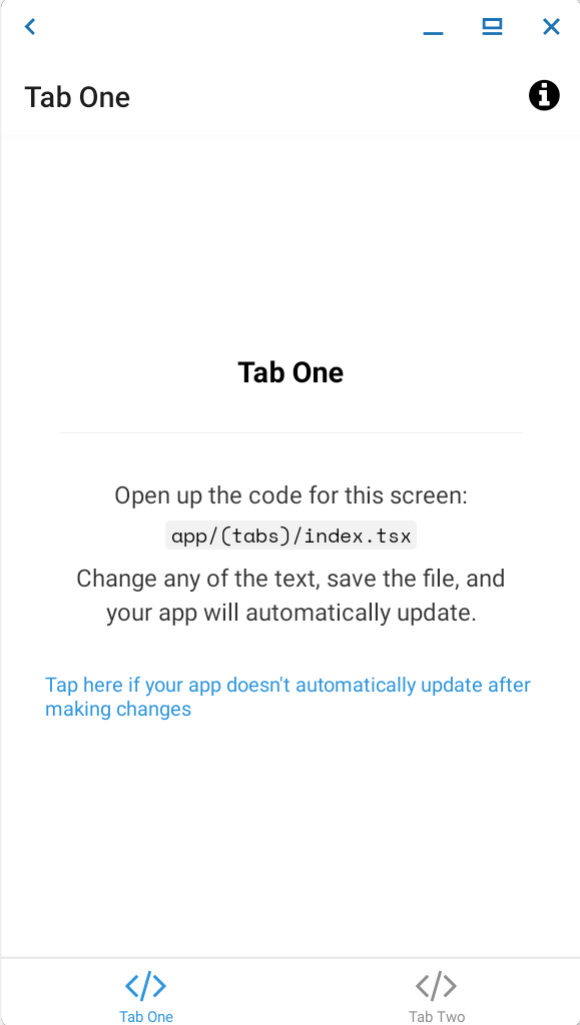
\includegraphics[width=\linewidth, frame]{implementation/second iteration/ca5b6d244e53f298ad7fe0d304d3591698032a39.png}
    \label{fig:wrapfig}
  \end{wrapfigure}

  \noindent \\ We can preview our changes in real-time on an iOS or Android device by running \lstinline{npx expo start}.
  If we run this command now we can see the generated boilerplate code in action on the right:

  \noindent \\ Below is the function generated by
  \lstinline{create-expo-app} that renders this page.

  \begin{lstlisting}[language=typescript, breaklines=false]
      // Imports omitted

      export default function TabOneScreen() {
        return (
          <View style={styles.container}>
            <Text style={styles.title}>Tab One</Text>
            <View
              style={styles.separator}
              lightColor="#eee"
              darkColor="rgba(255,255,255,0.1)"
            />
            <EditScreenInfo path="app/(tabs)/index.tsx" />
          </View>
        );
      }

      // Styling omitted
    \end{lstlisting}

\end{dummyenv}

\subparagraph{A note regarding syntax\\}

\noindent \\ The HTML-like syntax inside the
\lstinline[language=typescript]{return ()} block is an example
of TSX (or JSX for JavaScript). JSX and TSX stand for JavaScript
and TypeScript XML respectively, allowing the programmer
to use XML (including, but not limted to HTML tags) inside of JS/TS.
It uses a 'x' suffix on the file extension in order
to distinguish between eg. plain TypeScript and TSX.
(eg \lstinline{file.ts} becomes \lstinline{file.tsx})

\noindent \\ You may also notice that some tags do not
appear to be standard HTML. This is because TSX/JSX can also contain
React components (eg. \lstinline[language=tsx]{<View />}).
This will be explained in the next section.
In addition, while not shown in this example, JSX/TSX
can use inline JavaScript/TypeScript inside of an XML tag at any time
by using curly brackets. In conclusion:

%\noindent \\ On the surface, JSX syntax is remarkably similar to
%that of HTML, but with two key differences:

\begin{enumerate}
  \item React features custom elements called "components" (eg. \lstinline[language=tsx]{<View />})
  \item TSX/JSX can have inline JavaScript/Typescript by using curly brackets, eg:
        \begin{enumerate}
          \item \lstinline[language=typescript]|<Button onClick={/* js/ts code here */} />|
          \item \lstinline[language=typescript]|<Button onClick={() => alert("Hello, world!")} />|
                \begin{itemize}
                  \item[\labelitemi] In this example, we are using an
                        ES6 \underline{anonymous function} which creates
                        a pop-up box saying "Hello, world!"
                \end{itemize}
        \end{enumerate}
\end{enumerate}

% \subsubsection{Integrating the Apollo GraphQL client for backend communication}

\begin{dummyenv}
  \begin{wrapfigure}{r}[25pt]{0.4\textwidth}
    \begin{framed}{}
      \resizebox{\textwidth}{!}{
        \begin{tikzpicture}[node distance=2cm]
          \node (start) [startstop] {Start};

          % Constructor section
          %\node[align=center] (init) [process, below of=start] {Constructor\\is called};
          \node[align=center] (init_1) [process, below of=start, yshift=-1cm] {Component\\props are set};
          \node[align=center] (init_2) [process, below of=init_1] {Initial component\\state is set};
          % surrounding box
          \node[thick, draw=red,fit=(init_1) (init_2)] (init_box) {};
          \node[text=red, above of=init_box, align=left, yshift=0.5cm, xshift=1.5cm] (init_text) {Constructor\\ is called};


          \node[align=center] (render1) [io, below of=init_2] {\lstinline{(initial)\\render()}\\called};
          \node[align=center] (did_mount) [process, below of=render1] {\lstinline{componentDidMount()}\\called};
          \node[align=center] (should_update) [process, below of=did_mount] {\lstinline{shouldComponentUpdate()}\\called};
          \node[align=center] (render2) [io, below of=should_update] {\lstinline{render()}\\called};
          \node[align=center] (did_update) [process, below of=render2] {\lstinline{componentDidUpdate()}\\called};

          % positioning
          \node[inner sep=0pt, right of=should_update, xshift=1cm] (pos1) {};
          \node[inner sep=0pt, right of=did_update, xshift=1cm] (pos2) {};

          \draw [arrow] (start) -- (init_1);
          \draw [arrow] (init_1) -- (init_2);
          \draw [arrow] (init_2) -- (render1);
          \draw [arrow] (render1) -- (did_mount);
          \draw [arrow] (did_mount) -- (should_update);
          \draw [arrow] (should_update) -- (render2);
          \draw [arrow] (render2) -- (did_update);
          \draw [arrow] (did_update.east) -- (pos2) -- (pos1) -- (should_update);

          % redo arrow text
          \node[right of=render2, xshift=2cm,  align=left] (redo_text) {State\\changes};
        \end{tikzpicture}
      }

      \caption{
        \centering
        React component\\
        lifecycle diagram (simplified)
      }
    \end{framed}
    \label{fig:wrapfig}
  \end{wrapfigure}

  \paragraph{} % newline otherwise tikz doesn't show up

  \subsubsection{React Components}

  \noindent React Components allow the programmer to split up the React tree.

  \noindent \\ The headline feature of React Components is
  the ability to nest them. This introduces us to the concept
  of parent and child components.

  \subparagraph{Component lifecycle\\}

  \noindent \\ The flowchart on the right shows a simplified version of the lifecycle
  of a React component. The component lifecycle begins with the component's constructor
  being called, which sets it's props and state. Component props are the arguments passed to
  a React component, which can be done like so:
  \lstinline[language=typescript]{<CustomComponent prop="value" />}
  In this instance, prop is the paramater and "value" is the value.

  \noindent \\ A component's state is where component properties are traditionally stored.
  This is because, as can be seen on the right, when a component's state changes, a re-render
  of the component occurs.

  \subparagraph{Nesting React Components\\}

  \noindent \\ In order to nest a React Component, we use the specially assigned
  \lstinline{children} prop. For example, if we do the following:

  \begin{lstlisting}[language=typescript]
    <ParentComponent>
      <ChildComponent/>
    </ParentComponent>
  \end{lstlisting}
\end{dummyenv}

% end of inline space
\noindent Then ParentComponent's \lstinline{children} prop is set to
\lstinline{<ChildComponent/>}.

\noindent However, this alone will not make ChildComponent render. In order to do this,
we need to do the following inside of ParentComponent:

\begin{lstlisting}[language=typescript]
  const ParentComponent = ({ children }) => {
    return (
      <>
        {children}
      </>
    )
  }
\end{lstlisting}

\noindent \\ This will cause ParentComponent to return any children,
causing the children to render.

\noindent \\ \textbf{Note:} When a React app is rendered, the first node,
known as the root node, is rendered first.


\subsubsection{Researching React hooks and context}


As mentioned previously, the client (frontend component) and server (backend component)
will communicate using GraphQL. \textbf{Apollo Client} is a GraphQL client designed for use with
React and React Native. It can be installed using
\lstinline[language=bash]{npm install @apollo/client graphql}.


% SKIP for now: (frontend/metro):  Allow mjs files to be imported to make graphql package work

\noindent \\ Apollo now needs to be connected to the backend service.
In order to achieve this, I needed to learn about two React features:

\begin{enumerate}
  \item \textbf{React hooks} are functions that allow a developer
        to "hook into" different events during a different lifecycle stages
        of a React component, such as before and after the initial render.

  \item \textbf{React context} are hooks that allow a developer
        to share information between different components in the tree.
        A React Context makes available an asynchronous function that
        can be called from any child component to access shared variables.
\end{enumerate}

\noindent \\ After researching these features, I came to the following conclusion:

\begin{itemize}
  \item React hooks are useful as it allows components to render differently on the first render
        \begin{itemize}
          \item eg. to show a loading page ont the first render
        \end{itemize}
  \item However, certain React hooks such as context are not
        available until after the first render.
        \begin{itemize}
          \item I will come back to this in Section TODO.
        \end{itemize}
\end{itemize}

\paragraph{React Context\\}

\noindent \\ React Context would allow me to initialize Apollo Client once,
and share the instance between all child objects. This would be useful as
all objects in React including the different screens in an application share a common
root component at the top of the tree. If I was to initialise Apollo Client
before the navigation component (from \lstinline{expo-router}) I would be able to access
the client from any screen in the application. This was the approach I chose to take.

\noindent \\ I used the following code to create a React context:

\begin{lstlisting}[language=typescript, numbers=left, framesep=6pt]
  type JwtToken = {
    jwt: string | null,
    isLoading: boolean
  } | null

  const AuthContext = React.createContext<{
    login: (email: string, password: string) => Promise<LoginData | null | undefined>,
    logout: () => void,
    getCreds: () => Promise<boolean>,
    access: JwtToken,
    refresh: JwtToken,
  }>({
    login: async (email: string, password: string) => null,
    logout: () => null,
    getCreds: async () => false,
    access: null,
    refresh: null
  })
\end{lstlisting}

\noindent \\ Lines 6-18 define a React Context. Three functions are
defined in lines 7-9, \lstinline{login}, \lstinline{logout} and
\lstinline{getCreds}.
The first and third functions are \textbf{asynchronous}.
In TypeScript this means that the function returns a
\lstinline[language=typescript]{Promise}, a function that must be
\textbf{awaited} in order to execute it.

\noindent Lines 10-11 define two variables which will be made accessible to
child components, \lstinline{access} and \lstinline{refresh}.
% global btw
These two variables are of type \lstinline{JwtToken}, defined on
lines 1-4. As defined on lines 1-4, a variable of type
\lstinline{JwtToken} is an \underline{optional variable} that is
\textbf{either} \lstinline{null} \textbf{or} an object containing
two variables, \lstinline{jwt} (string \textbf{or} null) and
\lstinline{isLoading},a boolean that is either true or false.
Since TypeScript, unlike JavaScript, is a strongly
typed language, we must define types for all variables, or set
the type to \lstinline{any}.
Lines 13-17 define the default values of the functions and variables,
setting them all to null. The values will be set when the context
is added to the node tree (rendered inside a component)

\subsubsection{Setting up a Authentication Provider}

\noindent \\ In order to use the \lstinline{AuthContext} I had
created, I would need to create a React Component that contained it,
so that it would be a part of the React Tree.

%\paragraph{Nesting React Components\\}



\begin{comment}
\paragraph{Configuring Apollo Client to talk to the backend component}


\begin{lstlisting}[language=typescript]
  // Define a hook to be called within SessionProvider to access the session
  export function useSession() {
    const value = React.useContext(AuthContext)

    if (process.env.NODE_ENV !== 'production') {
      if (!value) {
        throw new Error('useSession must be wrapped in a <SessionProvider />');
      }
    }
    return value;
  }
\end{lstlisting}
\end{comment}

\end{document}